\section{Učenje SSD neuronske mreže}
\subsection{Visoki pogled na učenje}
Bitna razlika u učenju \emph{SSD} mreže i tipične \emph{R-CNN} mreže slične zadaće je ta da "ground truth" podatak mora biti dodjeljen točnom izlazu iz fiksnog skupa izlaza detektora \cite{liu2016ssd}.
Na sličan način radi i veliko poboljšanje na \emph{R-CNN} arhitekturu, \emph{Faster R-CNN}. \\
Kao i kod klasičnih neuronskih mreža, primjenjuje se funkcija gubitka, a za određivanje težina koristi se tehnika \emph{back propagation}.
Prije početka učenja također se određuju pretpostavljeni pravokutnici, različite skale za detekciju i strategije za povećanje podataka. \\
O pretpostavljenim kvadratima, skalama za detekciju i strategijama pisati će se u nastavku.
\subsection{Određivanje pozicije objekata}
Tijekom učenja, cilj je odrediti koji pretpostavljeni pravokutnici najbolje odgovaraju "ground truth" pravokutnicima objekta, to jest onima specifiranim u skupu podržavamotaka.
Nakon što se odrede najprecizniji pravokutnici, mreža se sukladno tome dalje prilagođava.
Za svaki "ground truth" pravokutnik imamo na izbor više pretpostavljenih pravokutnika, različitih lokacija, skala i omjera.
Želimo naći onaj koji ima najveći \emph{jaccardov index preklapanja} (dalje \emph{IoU}) (slika ~\ref{fig:JaccardIndex}) \cite{SSD}.
\begin{figure}[h!]
	\centering
	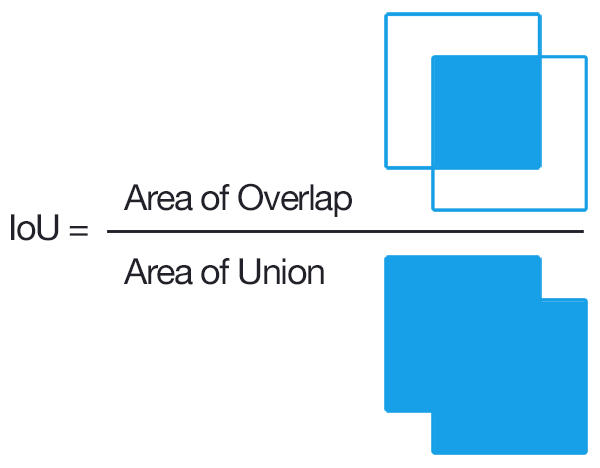
\includegraphics[width=0.6\linewidth]{iou_equation}
	 \caption{Način na koji računamo \emph{jaccardov index preklapanja, tj. IoU}.}
 	 \label{fig:JaccardIndex}
\end{figure} \\
U konfiguracijskoj datoteci koja će biti priložena na kraju rada, možemo ručno odrediti od koje preciznosti pretpostavljeni pravokutnik prihvačamo.
Pretpostavljena vrijednost je da mora vrijediti $IoU \geq 0.5$.
To višestruko olakšava treniranje jer mreža zadržava više pretpostavljenih pravokutnika umjesto da mora odabrati samo onaj sa najvećim preklapanjem.
\subsection{Određivanje parametara za nastavak učenja}
Određivanje parametara bilo bi puno lakše kada bismo imali samo jedan objekt za klasificirati, no postaje kompliciranije uz više objekata.
Uzmimo $x^p_{ij}=\{1,0\}$ kao indikator za podudaranje $i$-tog pretpostavljenog pravokutnika na $j$-ti "ground truth" pravokutnik kategorije $p$.
Koristeći spomenutu strategiju određivanja pozicije objekata može nam se dogoditi situacija $\sum_i{x_{ij}^p} \geq 1$. \\
Ukupna funkcija gubitka računa se kao otežana suma lokalizacijskog (\emph{loc}) i klasifikacijskog (\emph{conf}) gubitka \cite{liu2016ssd}:
\begin{equation}
	\label{eq:lokKlasLoss}
	L(x,c,l,g)=\frac{1}{N}(L_{conf}(x,c)+\alpha L_{loc}(x,l,g))
\end{equation}
$N$ nam predstavlja broj "pogođenih" pretpostavljenih pravokutnika. Naravno, ako je $N=0$, postavimo da je gubitak također $=0$.
\subsubsection{Lokalizacijski gubitak (\emph{loc})}
Za izračun lokalizacijskog gubitka koristimo \emph{Smooth L1} između predviđenih i "ground truth" pravokutnika \cite{liu2016ssd}.
\begin{equation}
	\label{eq:lokLoss}
	L_{loc}(x,l,g)=\sum_{i\in Pos\ m \in\ (cx, cy, w, h)}^{N} \ \sum x_{ij}^k\ smooth_{L1}(l_i^m - \hat g_j^m)
\end{equation}
\subsubsection{Klasifikacijski gubitak (\emph{conf})}
Klasifikacijski gubitak računa se kao \emph{softmax} svih klasa koje podržavamo \cite{liu2016ssd}.
\begin{equation}
	\label{eq:klasLoss}
	L_{conf}(x,c)=-\sum_{i \in Pos}^N x_{ij}^p \log(\hat c_i^0) - \sum_{i \in Neg} \log(\hat c_i^0 ) \ {gdje} \ \hat c_i^p=\frac{\exp(c_i^p)}{\sum_p \exp(c_i^p)}
\end{equation}
\subsection{Definiranje trajanja učenja}
Tijek i trajanje učenja može se opisati koristeći više parametara. 
Korišteni \emph{Tensorflow object detection API} zahtjeva određivanje broja koraka, dok se u litraturi, npr. \cite{chollet2017deep}  najčešće koristi epoha.
\subsubsection{Korak}
Mreži se u konfiguracijskoj datoteci, priloženoj na kraju rada predaje parametar \emph{batch size}.
\emph{Batch size} definira koliko će se u jednom trenutku uzeti slika za učenje.
Parametar, iako može biti jedan, najčešće je 24 \cite{tensorflow.org}.
Nakon što mreža obradi sve slike uzete u jednom trenutku ona popravlja svoje parametre, odnosno težine.
Upravo to razdoblje od uzimanja određenog broja slika, i obrade svih definira \emph{korak}.
Koliko korak traje?
Učenje mreže za ovaj rad izvodilo se na dva uređaja zbog potrebe mjerenja i vidljivo je na tablici ~\ref{tab:uredaji} koja prikazuje povezanost procesnih jedinica uređaja na kojima se učenje vršilo i pripadajuća vremena po jednom koraku treniranja.
\begin{center}
	\begin{tabular}{||c c||}
		\hline
		Specifikacije uređaja & Vrijeme po koraku (s) \\ [0.5ex]
		\hline\hline
		Macbook Pro 2016, Intel i5 2.9GHz, 8GB & 13.57 \\
		\hline
		ZEMRIS C22, NVidia GTX 1080 Ti, 11GB & 0.86 \\ [1ex]
		\hline
	\end{tabular}
\label{tab:uredaji}
\end{center}
\subsubsection{Epoha}
Epoha označava pregled cijelog skupa podataka. 
To naravno ne znači da je svaka slika pogledana točno jednom jer su nasumično učitavane u mrežu ali onaj trenutak kada su sve barem jednom prošle kroz mrežu označava kraj jedne epohe.
Uz pretpostavku da je svaka slika pogledana jednom, približno se može izračunati broj epoha iz broja koraka formulom ~\ref{eq:stepEpoch}.
\begin{equation}
	\label{eq:stepEpoch}
	broj epoha = brojKoraka \times \frac{batchSlika}{brojSlika}
\end{equation}
